% Created 2019-11-02 Sat 07:46
\documentclass[11pt]{article}
\usepackage[utf8]{inputenc}
\usepackage[T1]{fontenc}
\usepackage{fixltx2e}
\usepackage{graphicx}
\usepackage{longtable}
\usepackage{float}
\usepackage{wrapfig}
\usepackage{rotating}
\usepackage[normalem]{ulem}
\usepackage{amsmath}
\usepackage{textcomp}
\usepackage{marvosym}
\usepackage{wasysym}
\usepackage{amssymb}
\usepackage{hyperref}
\tolerance=1000
\author{Hack Chyson}
\date{\today}
\title{note}
\hypersetup{
  pdfkeywords={},
  pdfsubject={},
  pdfcreator={Emacs 25.2.1 (Org mode 8.2.10)}}
\begin{document}

\maketitle
\tableofcontents

\section{Preface}
\label{sec-1}
Algorithms lies at the heart of computering. \\

Website: \url{http://mitpress.mit.edu/algorithms/} \\

Psudocode: present algorithm clearly and succintly, without idiosyncrasies of a particular programming language obscuring the its essence. \\

\section{Foundations}
\label{sec-2}
\subsection{The Role of Algorithms in Computing}
\label{sec-2-1}
\subsubsection{what is algorithm?}
\label{sec-2-1-1}
input -> algorithm -> output \\
An algorithm is a sequence of computational steps that transform the input into the output. \\
A algorithm describes a specific computational procedure for achieving the input/output relationship. \\

\subsubsection{instance of a problem}
\label{sec-2-1-2}
the input needed to compute a solution to the problem. \\

\subsubsection{correct algorithms}
\label{sec-2-1-3}
For every input instance, it halts out the correct output. \\

\subsubsection{problem list}
\label{sec-2-1-4}
\begin{itemize}
\item Internet, finding good routes and finding pages \\
\item Electronic commerce, public-key cryptography and digital singatures \\
\item oil company, where to place its wells in order to maximize its profit, linear programming \\
\item road map, shortest route \\
\item two ordered sequences, find a longest common subsequence \\
\item a mechanical design, each part may include instances of other parts, to list the parts in order so that each part appears before any part that uses it, topological sorting \\
\item convex hull \\
\end{itemize}

\subsubsection{two characteristics of many algorithms}
\label{sec-2-1-5}
\begin{enumerate}
\item There are many candidate solutions, but finding the one that solve or the one is best is challenge. \\
\item They have practical applications. \\
\end{enumerate}

\subsubsection{data structure}
\label{sec-2-1-6}
a way to store and organize data in order to facilitate access and modifications. \\

No single data structure works well for all purposes, and it is important to know the strengths and limitations of several of them. \\

\subsubsection{the core technique}
\label{sec-2-1-7}
learn the technique of algorithm design and analysis. \\

\subsubsection{hard problems}
\label{sec-2-1-8}
Like the NP-complete problem, there are problem that has no efficient solutions. \\
Before you delve into the real problem, take a overview of it. \\

\subsubsection{NP-complete problem}
\label{sec-2-1-9}
\begin{enumerate}
\item no one knows whether or not efficient algorithms exist. \\
\item a solution for one NP-complete probelm will works for all NP-complete problems \\
\item several NP-complete problems are similar, but not identical to problems for which we do know of efficient algorithms. \\
\end{enumerate}

\subsubsection{algorithm efficiency}
\label{sec-2-1-10}
Computers are not infinitely fast and memory is not free, thus the efficiency of a algorithm matters. \\
\textit{[2019-06-21 Fri]} \\
\subsubsection{algorithms as a technology}
\label{sec-2-1-11}
Algorithms are at the core of most technologies. \\


\textit{[2019-06-22 Sat]} \\
\subsection{Getting Started}
\label{sec-2-2}
\subsubsection{loop invariant}
\label{sec-2-2-1}
Loop invariant is used to help us to understand why an algorithm is correct. \\

The comparison of loop invariant and mathematical induction \\
\begin{center}
\begin{tabular}{|l|l|}
\hline
Loop Invariant & Mathematical Induction \\
\hline
initialization & base case \\
\hline
maintenance & inductive step \\
\hline
termination & \\
\hline
\end{tabular}
\end{center}

Initialization: It is true prior to the first iteration of the loop. \\
Maintanance:    If it is true before an iteration of the loop, it remains true before the next iteration. \\
Termination:    When the loop terminates, the invariant gives us a useful property that helps show that the algorithm is correct. \\
\subsubsection{psudocode conventions}
\label{sec-2-2-2}
\begin{verbatim}
INSERTION-SORT(T)

for j = 2 to A.length
    key = A[j]
    // Insert A[j] into the sorted sequence A[1..j-1].
    i = j - 1
    while i > 0 and A[i] > key
        // in place sort
        A[i + 1] = A[i]
	i = i - 1
    // when the loop terminate, i = 0
    A[i + 1] = key
\end{verbatim}


\begin{enumerate}
\item Indentation indicates block structures. \\
\item A loop counter retains its value after exiting the loop. (deffer from C++, Java\ldots{}) \\
\item Variable are local to the given procedure. \\
\item The keyword \textbf{error} indicates that an error occurred. \\
\end{enumerate}




\subsubsection{analyzing algorithms}
\label{sec-2-2-3}
analyzing an algorithm: predict the resources. \\
resources: time and space (memory, communication bandwidth, computer hardware, computational time\ldots{}) \\

\subsubsection{model}
\label{sec-2-2-4}
Before analyzing an algorithm, there must be a model to measure the resource cost. \\

\subsubsection{algorithm vs RAM}
\label{sec-2-2-5}
The focus is algorithm, not the tedious hardware detail. \\
To yield a clear insight into algorithm design and analysis, RAM model is simplified. \\

\subsubsection{RAM model}
\label{sec-2-2-6}
\begin{center}
\begin{tabular}{|l|l|l|l|l|}
\hline
instructions & arithmetic & movement & control & \\
\cline{2-4}
 & add, abstruct, & load, store copy & conditional and & each instructions takes \\
 & multiply, & & unconditional & a constant amount of \\
 & divide, & & branch, & time \\
 & remainder, & & subroutine call, & \\
 & floor, ceiling & & return & \\
 & & & & \\
\hline
data types & \multicolumn{3}{l|}{integer, floating} & represented by clgn \\
 & \multicolumn{3}{l|}{} & bits \\
\hline
memory hierarchy & \multicolumn{3}{l|}{do not model caches or virtual memory} & \\
\hline
\end{tabular}
\end{center}

$c\lg n$ explaination: \\
\begin{itemize}
\item $\lg$ means $\log_2$ \\
\item 2 as root because of the binary system \\
\item $c\ge1$ : each word can hold the value of n \\
\item $c$ to a constant: the word size does not grow arbitrarily \\
\end{itemize}

\subsubsection{core idea in modeling}
\label{sec-2-2-7}
show tha important characteristcs of algorithms and suppress the tedious details. \\



\subsubsection{analysis of a algorithm}
\label{sec-2-2-8}
In general, the time grows with the size of the input, \\
so it is traditional to describe the running time as the function of the size of its input. \\

\begin{center}
\begin{tabular}{|l|l|l|}
\hline
 & & Examples \\
\hline
input size & depends on the problem being studied & number of items, total number of bits ... \\
\hline
running time & the number of primitive operations & \\
\hline
\end{tabular}
\end{center}

Assumption for simpler analysis: \\
A constant amount of time is requried to execute each line of the pseudocode. \\



\subsubsection{worst-case analysis}
\label{sec-2-2-9}
Becuase the behavior of an algorithm may be different for each possible input, \\
we need a means for summarizing that behavior in simple, easily understood formulas. \\


the reason to analyze worst-case running time: \\
\begin{enumerate}
\item give an upper bound on the running time \\
\item worst case ocurrs fairly often \\
\item the "average case" is often roughly as bad as the worst case \\
\end{enumerate}

\subsubsection{abstraction}
\label{sec-2-2-10}
Use some simplifying abstraction to ease the analysis. \\
\begin{enumerate}
\item ignore the actual cost of each statement, using the constants $c_i$ to represent these costs. \\
\item ignore the abstract costs $c_i$ ( $an^2 + bn + c$ ) \\
\item rate of growth or order of growth of the running time ( $\Theta(n^2)$ ) (pronounced "theta of n-squared") \\
\end{enumerate}


\subsubsection{designing algorithms}
\label{sec-2-2-11}
\begin{enumerate}
\item incremental approch
\label{sec-2-2-11-1}
example: insertion-sort \\
\item devide-and-conquer approch
\label{sec-2-2-11-2}
example: like merge-sort \\

\begin{enumerate}
\item divide the problem into a number of subproblems \\
\item conquer the subproblems \\
\item combine the solution \\
\end{enumerate}
\end{enumerate}


\subsection{Growth of Functions}
\label{sec-2-3}
Althoght we can sometimes determine the exact running time of an algorithm, the extra procision is not usually worth the effort of computing it. \\


When we look at input sizes large enought to make only the order of growth of the running time relevant, we are studying the \texttt{asymptotic efficiency of algorithms}. \\
\subsubsection{Asymptotic notation}
\label{sec-2-3-1}
\begin{enumerate}
\item $\Theta$-notation
\label{sec-2-3-1-1}
\begin{equation}

\Theta(g(n)) = \{f(n): \text{there exist positive constant}\ c_1, c_2 \text{and} \ n_0 \text{such that} \
0 \le c_1 g(n) \le f(n) \le c_2 g(n)\  \text{for all} \ n \ge n_0 \}
\end{equation}

Because $\Theta(g(n))$ is a set, we could write "$f(n) \in \Theta(g(n))$ " to indicate that $f(n)$ is a member of $\Theta(g(n))$ . Instead, we will usually write "$f(n) = \Theta(g(n))$ " to express the same notion. \\

Since any constant is a degree-0 polynomial, we can express any constant function as $\Theta(n^0)$ , or $\Theta(1)$ . \\
\item O-notation
\label{sec-2-3-1-2}
\begin{equation}
O(g(n)) = \{f(n): \text{there exist positive constants} \ c \text{and} \ n_0 \ \text{such that} \\
0 \le f(n) \le cg(n) \ \text{for all} \ n \ge n_0 \}
\end{equation}

O-notation to the worst case ==> to every input \\
$\Theta$-notation to the worst case =/=> to every input \\
\item $\Omega$-notation
\label{sec-2-3-1-3}
\begin{equation}
\Omega(g(n)) = \{f(n): \text{there exist positive constants} \ c \text{and} \ n_0 \ \text{such that} \
0 \le cg(n) \le f(n) \ \text{for all} \ n \ge n_0 \}
\end{equation}
\item Theorem
\label{sec-2-3-1-4}
For any two functions $f(n)$ and $g(n)$, we have $f(n) = \Theta(g(n))$ if and only if \\
$f(n) = O(g(n))$ and $f(n) = \Omega(g(n))$ \\
\item o-notation
\label{sec-2-3-1-5}
an upper bound that is not asymptotically tight. \\

\begin{equation}
o(g(n)) = \{f(n): \text{for any positive constant} \ c > 0, \text{there exist a constant} \ n_0 > 0 \ \text{such that} \
0 \le f(n) < cg(n) \ \text{for all} \ n \ge n_0 \}
\end{equation}


or \\
\begin{equation}
\lim_{n\rightarrow \infty}\frac{f(n)}{g(n)} = 0
\end{equation}

\item $\omega$-notation
\label{sec-2-3-1-6}
a lower bound that is not asymptotically tight. \\

\begin{equation}
\omega(g(n)) = \{f(n): \text{for any positive constant} \ c > 0, \text{there exist a constant} \ n_0 > 0 \ \text{such that} \
0 \le cg(n) < f(n) \ \text{for all} \ n \ge n_0 \}
\end{equation}


or \\
\begin{equation}
\lim_{n\rightarrow \infty}\frac{f(n)}{g(n)} = \infty
\end{equation}

\item comparing functions
\label{sec-2-3-1-7}
\begin{enumerate}
\item Transitivity
\label{sec-2-3-1-7-1}
$$
f(n) = \Theta(g(n)) \quad \text{and} \quad g(n) = \Theta(h(n)) \Rightarrow f(n) = \Theta(h(n))
$$ \\
The same to $O, \Omega, o, \omega$ . \\

\item Reflexivity
\label{sec-2-3-1-7-2}
$$f(n) = \Theta(f(n))$$ \\
$$f(n) = O(f(n)) $$ \\
$$f(n) = \Omega(f(n)) $$ \\

\item Symmetry
\label{sec-2-3-1-7-3}
$$ f(n) = \Theta(g(n)) \quad \text{if and only if} \quad g(n) = \Theta(f(n)) $$ \\
\item Transpose symmetry
\label{sec-2-3-1-7-4}

$$ f(n) = O(g(n)) \quad \text{if and only if} \quad g(n) = \Omega(f(n)) $$ \\
$$ f(n) = o(g(n)) \quad \text{if and only if} \quad g(n) = \omega(f(n)) $$ \\
\end{enumerate}
\end{enumerate}
\subsubsection{Standard notations and common functions}
\label{sec-2-3-2}
\subsection{Divide-and-Conquer}
\label{sec-2-4}
A recurrence is an equation or inequality that describes a function in terms of its value on smaller inputs. \\

For example: \\
\begin{equation}
T(n)=
\begin{cases}
\Theta(1) & \mathbb{if} \quad n=1 \\
2T(n/2) + \Theta(n) & \mathbb{if} \quad n > 1
\end{cases}
\end{equation}

\subsubsection{The master method for solving recurrences}
\label{sec-2-4-1}
\begin{equation}
T(n)=aT(n/b)+f(n)
\end{equation}
where $a\ge 1$ and $b>1$ are constants and f(n) is an asymptotically positive function. \\

Then $T(n)$ has the following asymptotic bounds: \\
\begin{enumerate}
\item If $f(n) = O(n^{\log_b(a-\epsilon)})$ for some constant $\epsilon>0$, then $T(n)=\Theta(n^{\log_ba})$. \\
\item If $f(n) = \Theta(n^{\log_ba})$, then $T(n)=\Theta(n^{\log_ba}\lg n)$. \\
\item If $f(n) = O(n^{\log_b(a+\epsilon)})$ for some constant $\epsilon>0$, and if $af(n/b)\le cf(n)$ for some constant $c<1$ and all sufficiently large $n$, then $T(n)=\Theta(f(n))$. \\
\end{enumerate}

Intuitively, the larger of the two functions determines the solution to the recurrence. \\


Note: \\
Beyond this intuition, you need to be aware of some technicalities. In the first case, not only must $f(n)$ be smaller than $n^{\log_ba}$ , it must be polynomially smaller. In the third case, not only must $f(n)$ be larger than $n^{\log_ba}$ , it also must be polynomially larger and in addition satisfy the "regularity" condition that $af(n/b)\le cf(n)$ \\

\subsection{Probabilistic Analysis and Randomized Algorithms}
\label{sec-2-5}


Probabilistic analysis is the use of probability in the analysis of problems. \\

In order to perform a probabilistic analysis, we must use knowledge of, or make assumptions about, the distribution of the inputs. Then we analyze our algorithm, computing an average-case running time, where we take the average over the distribution of the possible inputs. Thus we are, in effect, averaging the running time over all possible inputs. When reporting such a running time, we will refer to it as the average-case running time. \\

we call an algorithm randomized if its behavior is determined not only by its input but also by values produced by a random-number generator. \\

In general, we discuss the average-case running time when the probability distribution is over the inputs to the algorithm, and we discuss the expected running time when the algorithm itself makes random choices. \\

\subsubsection{Indicator random variables}
\label{sec-2-5-1}
In order to analyze many algorithms, we use indicator random variables. Indicator random variables provide a convenient method for converting between probabilities and expectations. \\
Suppose we are given a sample space S and an event A. Then the indicator random variable $I\{A\}$ associated with event A is defined as \\
\begin{equation}
I\{A\}=
\begin{cases}
1 \quad \mathrm{if} \ A \ \mathrm{occurs} \\
0 \quad \mathrm{if} \ A \ \mathrm{does\ not\ occurs}
\end{cases}
\end{equation}

Lemma: \\
Given a sample space S and an event A in the sample space S, let $X_A = I\{A\}$. Then $E[X_A]=Pr\{A\}$. \\

\subsubsection{Randomized alogrithms}
\label{sec-2-5-2}
Most of the time, we do not have knowledge in the input distribution. Instead of assuming a distribution of inputs, we impose a distribution. \\

\begin{enumerate}
\item Randomly permuting arrays
\label{sec-2-5-2-1}
\begin{verbatim}
PERMUTE-BY-SORTING(A)
let P[1..n] be a new array
for i = 1 to n
    P[i] = RANDOM(1, n^3)  # priority
sort A, using P as sort keys
\end{verbatim}

\begin{verbatim}
RANDOMIZE-IN-PLACE(A)
n = A.length
for i = 1 to n
    swap A[i] with A[RANDOM(i, n)]
\end{verbatim}
\end{enumerate}

\section{Sorting and Order Statistics}
\label{sec-3}
sorting problem: \\

Input: A sequence of n numbers $a_1, a_2, ..., a_n$. \\
Output: A permutation (reordering) $a^'_1,a_2^',...,a_n^'$ of the input sequence such that $a_1^' \le a_2^' \le ... \le a_n^'$. \\

In practice, the numbers to be sorted are rarely isolated values. Each is usually part of a collection of data called a record. Each record contains a key, which is the value to be sorted. The remainder of the record consists of satellite data, which are usually carried around with the key. \\

\subsection{Heapsort}
\label{sec-3-1}

\subsubsection{Heaps}
\label{sec-3-1-1}
The (binary) heap data stucture is an array object that can view as nearly complete tree. Each node of the tree corresponds to an element of the array. The tree is completely filled on all levels except possibly the lowest, which is filled from the left up to a point. \\

An array A that represents a heap is an object with two attributes: \\
\begin{enumerate}
\item A.length, which gives the number of elements in the array \\
\item A.heap-size, which represents how many elements in the heap are stored with array A \\
\end{enumerate}

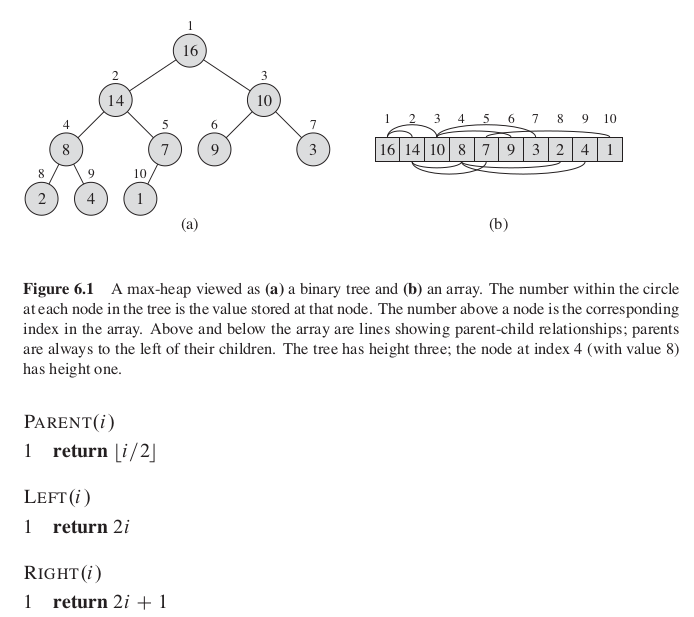
\includegraphics[width=.9\linewidth]{pics/c6_heap.png} \\

There are two kinds of binary heaps: max-heaps and min-heaps. In both kinds, the values in the nodes satisfy a heap property. \\

In a max-heap, the max-heap property is that for every node i other than root, $A[PARENT(i)] \ge A[i]$. \\
In a min-heap, $A[PARENT(i)] \le A[i]$. \\

\subsubsection{Maintaining the heap property}
\label{sec-3-1-2}
In order to maintain the max-heap property, we call the procedure MAX-HEAPIFY. Its inputs are an array A and an index i into the array. When it is called, MAX-HEAPIFY assumes that the binary trees rooted at LEFT(i) and RIGHT(i) are max-heaps, but that A[i] be smaller than its children, thus violating the max-heap property. \\

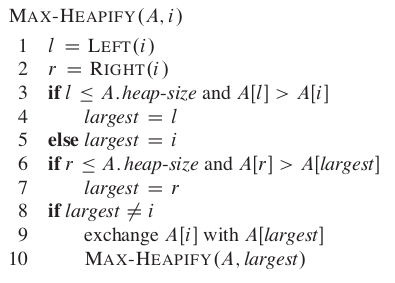
\includegraphics[width=.9\linewidth]{pics/c6_max_heapify.png} \\

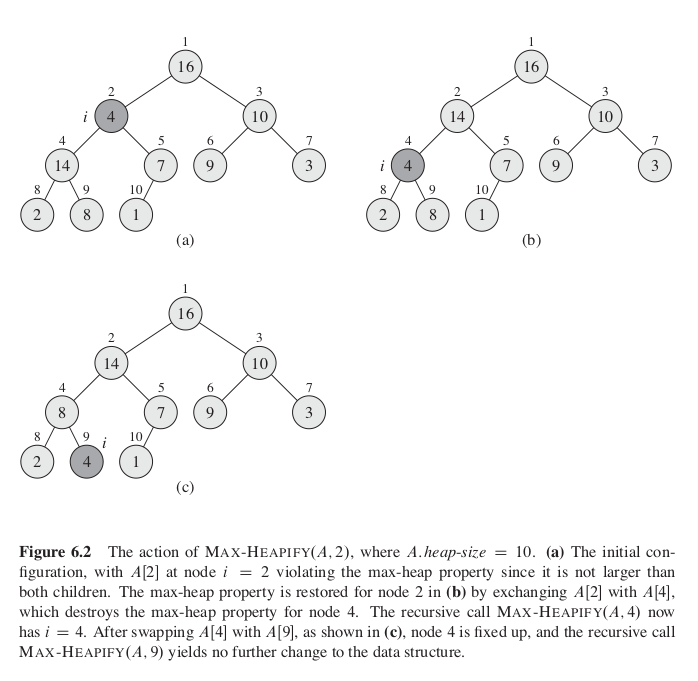
\includegraphics[width=.9\linewidth]{pics/c6_max_heapify_fig.png} \\

\subsubsection{Building a heap}
\label{sec-3-1-3}
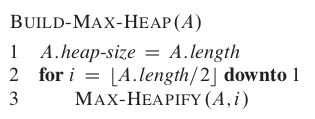
\includegraphics[width=.9\linewidth]{pics/c6_build_max_heap.png} \\


\subsubsection{The heapsort algorithm}
\label{sec-3-1-4}
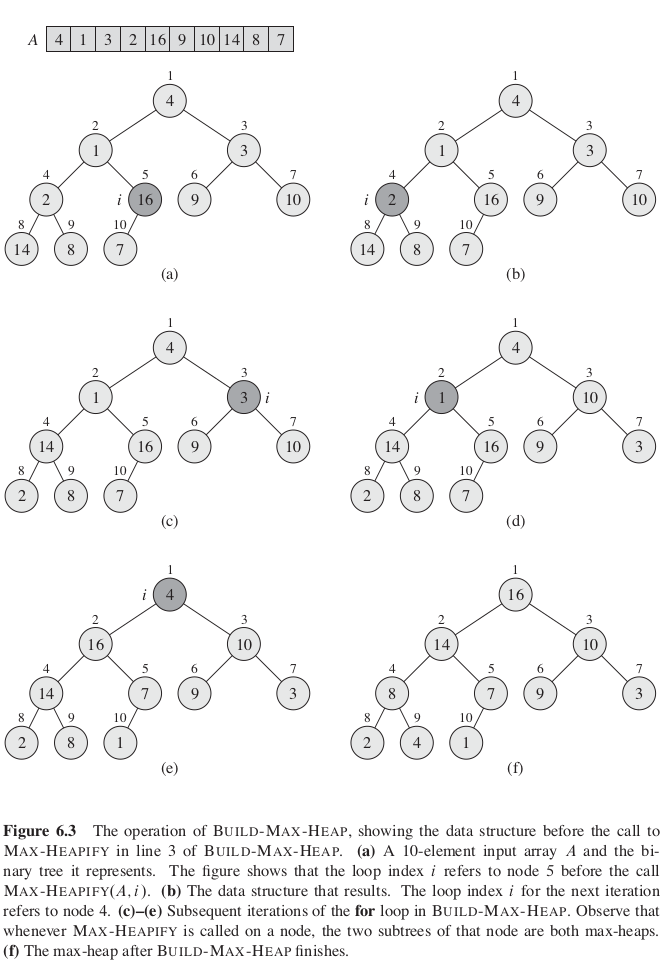
\includegraphics[width=.9\linewidth]{pics/c6_build_max_heap_fig.png} \\

\subsubsection{The heapsort algorithm}
\label{sec-3-1-5}
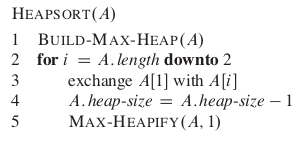
\includegraphics[width=.9\linewidth]{pics/c6_heapsort.png} \\

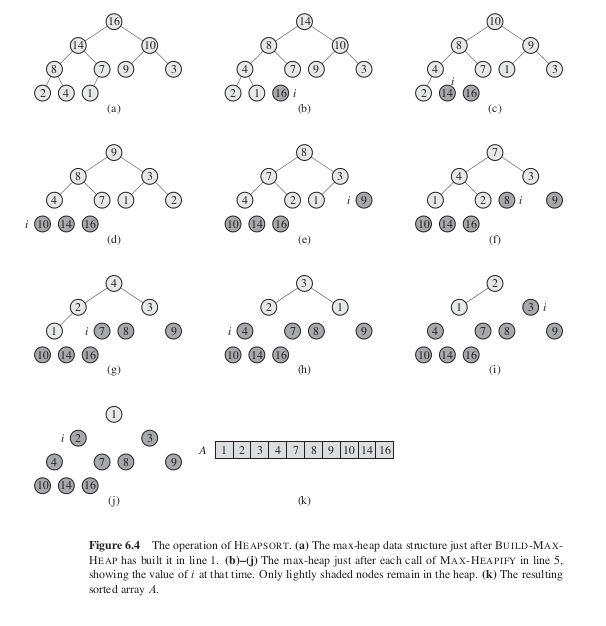
\includegraphics[width=.9\linewidth]{pics/c6_heapsort_fig.png} \\

\subsubsection{Priority queues}
\label{sec-3-1-6}
A priority queue is a data structure for maintaining a set S of elements, each with an associated value called a \textbf{key}. \\

A max-priority queue supports the following operations: \\
\begin{itemize}
\item INSERT(S,x) inserts the elements x into the set S, which is equivalent to the operations $S=S\cup \{x\}$. \\
\item MAXIMUM(S) returns the element of S with the largest key. \\
\item EXTRACT-MAX(S) removes and returns the element of S with the largest key. \\
\item INCREASE-KEY(S,x,k) increase the value of element x's key to the new value k, which is assumed to be at least as large as x's current key value. \\
\end{itemize}


When we use a heap to implement a priority queue, therefore, we often need to store a handle to the corresponding application object in each heap element. \\


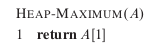
\includegraphics[width=.9\linewidth]{pics/c6_heap_maximum.png} \\

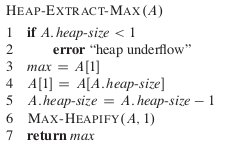
\includegraphics[width=.9\linewidth]{pics/c6_heap_extract_max.png} \\

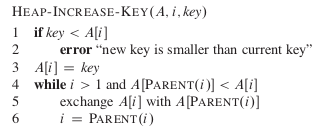
\includegraphics[width=.9\linewidth]{pics/c6_heap_increase_key.png} \\

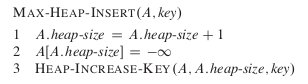
\includegraphics[width=.9\linewidth]{pics/c6_max_heap_insert.png} \\

\subsection{Quicksort}
\label{sec-3-2}
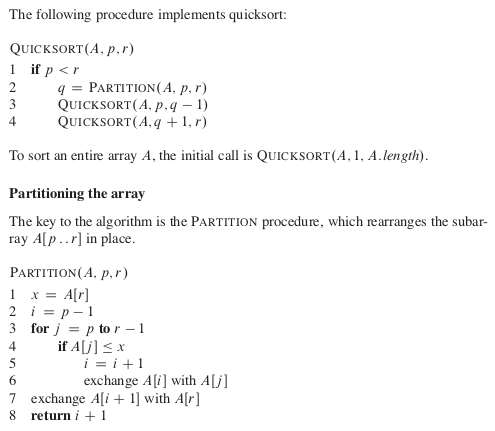
\includegraphics[width=.9\linewidth]{pics/c7_quicksort.png} \\

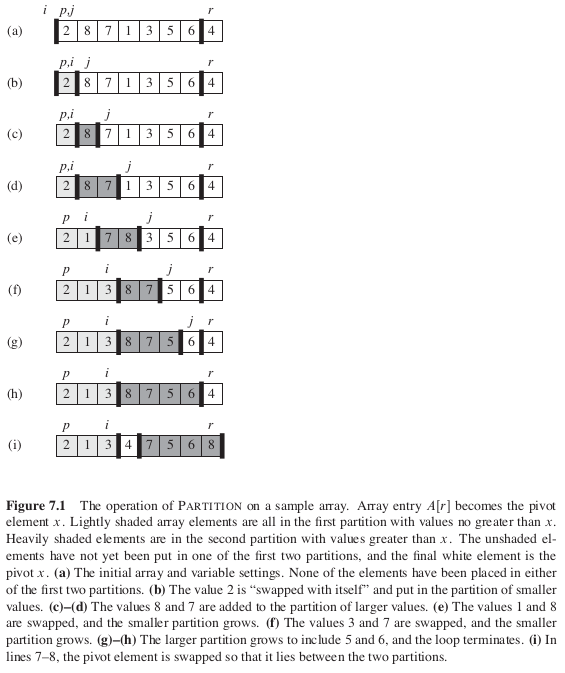
\includegraphics[width=.9\linewidth]{pics/c7_quicksort_fig.png} \\

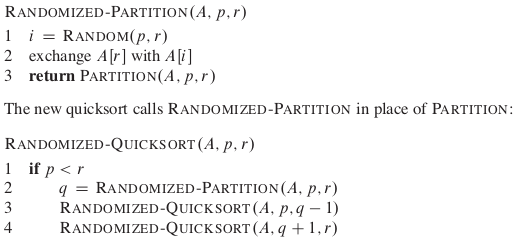
\includegraphics[width=.9\linewidth]{pics/c7_randomized_quicksort.png} \\

\subsection{Sorting in Linear Time}
\label{sec-3-3}
comparison sorts: the sorted order they determine is based only on comparison between the input elements. \\

Any comparison sort must make $\Omega(n\lg n)$ comparisons in the worst case to sort n elements. \\

\subsubsection{Counting sort}
\label{sec-3-3-1}
Counting sort assume that each of the input elements is a integer in the range 0 to k, for some integer k. When $k=O(n)$, the sort runs in $\Theta(n)$ time. \\

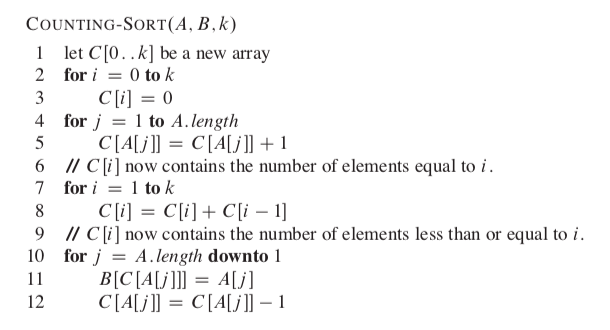
\includegraphics[width=.9\linewidth]{pics/c8_counting_sort.png} \\

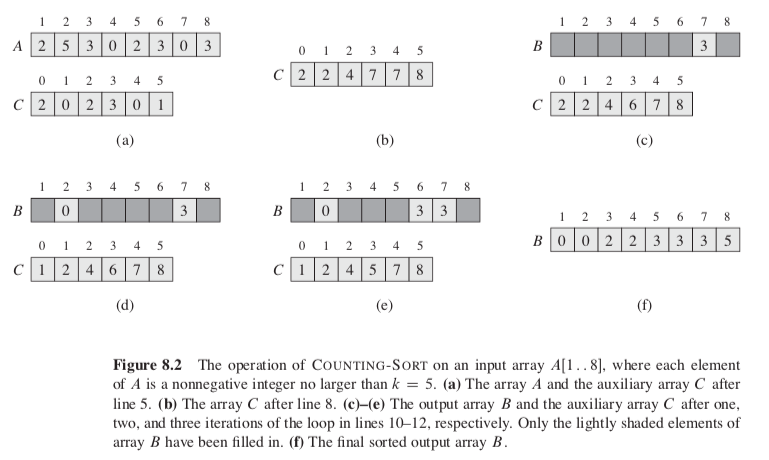
\includegraphics[width=.9\linewidth]{pics/c8_counting_sort_fig.png} \\

\subsubsection{Radix sort}
\label{sec-3-3-2}
The following procedure assumes that each element in the n-element array A has d digits, where digit 1 is the lowest-order digit and d is the highest-order digit. \\

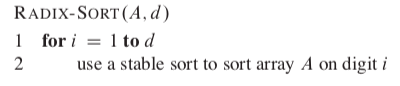
\includegraphics[width=.9\linewidth]{pics/c8_radix_sort.png} \\

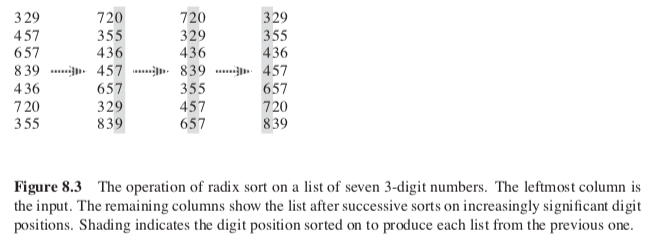
\includegraphics[width=.9\linewidth]{pics/c8_radix_sort_fig.png} \\

Given n d-digit numbers in which each digit can take on up to k possible values, RADIX-SORT correctly sorts these numbers in $\Theta(d(n+k))$ time if the stable sort it uses takes $\Theta(n+k)$ time. \\

\subsubsection{Bucket sort}
\label{sec-3-3-3}
Bucket sort assumes that the input is generated by a random process that distributes elements uniformly and independently over the interval [0,1). \\
Bucket sort divides the interval [0,1) into n equal-sized subintervals, or buckets, and then distributes the n inputs elements into the buckets. \\

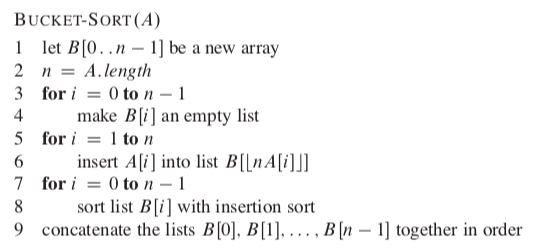
\includegraphics[width=.9\linewidth]{pics/c8_bucket_sort.png} \\

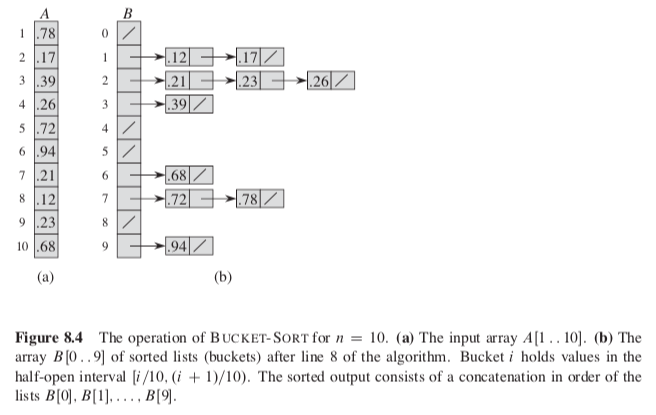
\includegraphics[width=.9\linewidth]{pics/c8_bucket_sort_fig.png} \\




\subsubsection{Medians and Order Statistics}
\label{sec-3-3-4}
The ith order statistic of a set of n elements is the ith smallest element. For example, the minimum of a set of elements is the first order statistics (i=1), and the maximum is the nth order statistics (i=n). \\
A median is the "halfway point" of the set. When n is odd, the median is unique, ocurring at $i=(n+1)/2$. When n is even, there are two median, ocurring at $i=\lfloor(n+1)/2\rfloor$ (the lower median) and $i=\lceil(n+1)/2\rceil$ \\


\section{Data Structures}
\label{sec-4}
In a typical implementation of a dynamic set, each element is represented by an object whose attributes can be examined and manipulated if we have a pointer to the object. \\

Operations on a dynamic set can be grouped into two categories: queries, which simply return information about the set, and modifying operations, which change the set. \\

SEARCH(S,k) \\
A query that, given a set S and a key value k, returns a pointer x to an element in S such that x.key = k, or NIL if on such element belongs to S. \\

INSERT(S,x) \\
A modifying operation that augements the set S with the element pointed to by x. \\

DELETE(S,x) \\
A modifying operation that, given a pointer x to an element in the set S, removes x from S. \\

MINIMUM(S) \\
A query on a totally ordered set S that returns a pointer to the element of S with the smallest key. \\

MAXIMUM(S) \\
A query on a totally ordered set S that returns a pointer to the element of S with the largest key. \\

SUCCESSOR(S,x) \\
A query that, given an element x whose key is from a totally ordered set S, returns a pointer to the next larger element in S, or NIL if x is the maximum element. \\

PREDECESSOR(S,x) \\
A query that, given an element x whose key is from a totally ordered set S, returns a pointer to the next smaller element in S, or NIL if x is the minimum element. \\

\subsection{Elementary Data Structure}
\label{sec-4-1}

\subsubsection{Stacks and queues}
\label{sec-4-1-1}
Stacks and queues are dynamic sets in which the element removed from the set by the DELETE operation is prespecified. In a stack, the element deleted from the set is the one most recently inserted: the stack implements a last-in, first-out, or LIFO, policy. Similarly, in a queue, the element deleted is always the one that has been in the set for the longest time: the queue implements a first-in, first-out, or FIFO, policy. \\

\begin{enumerate}
\item Stacks
\label{sec-4-1-1-1}
The INSERT operation on a stack is often called PUSH , and the DELETE operation, which does not take an element argument, is often called POP. \\

We can implement a stack of at most n elements with an array S[1..n]. The array has an attribute S.top that indexes the most recently inserted element. The stack consists of elements S[1..S.top], where S[ 1 ] is the element at the bottom of the stack and S[S.top] is the element at the top. \\

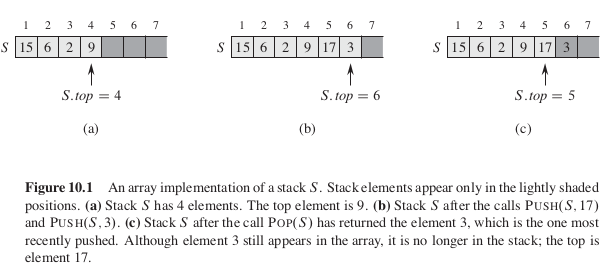
\includegraphics[width=.9\linewidth]{pics/c10_stack_fig.png} \\

When S.top = 0, the stack contains no elements and is empty. If we attempt to pop an empty stack, we say the stack underflows. If S.top exceeds n, the stack overflows. \\

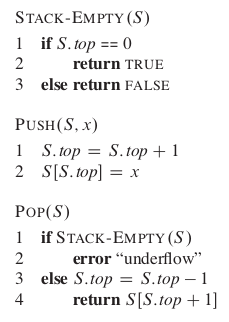
\includegraphics[width=.9\linewidth]{pics/c10_stack.png} \\

\item Queues
\label{sec-4-1-1-2}
We call the INSERT operation on a queue ENQUEUE , and we call the DELETE operation DEQUEUE. \\

The queue has a head and a tail. When an element is enqueued, it takes its place at the tail of the queue, takes a place at the end of the line. The element dequeued is always the one at the head of the queue. \\

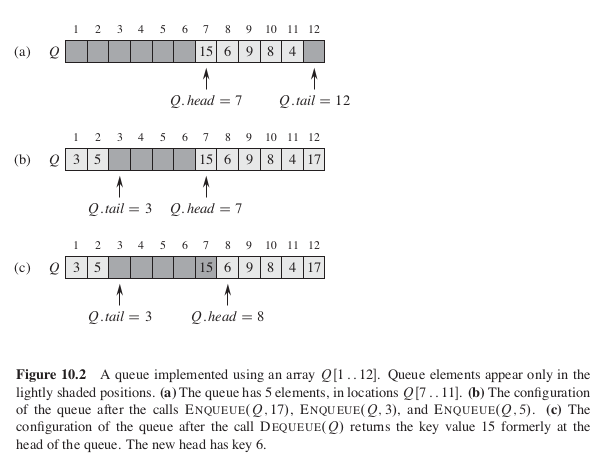
\includegraphics[width=.9\linewidth]{pics/c10_queue_fig.png} \\

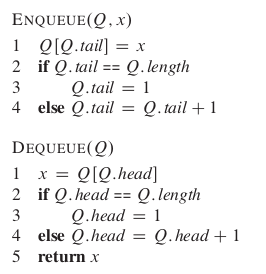
\includegraphics[width=.9\linewidth]{pics/c10_queue.png} \\
\end{enumerate}

\subsubsection{Linked lists}
\label{sec-4-1-2}
A linked list is a data structure in which the objects are arranged in a linear order. \\

\begin{verbatim}
Unlike an array, however, in which the linear order is determined by the array
indices, the order in a linked list is determined by a pointer in each object.
\end{verbatim}

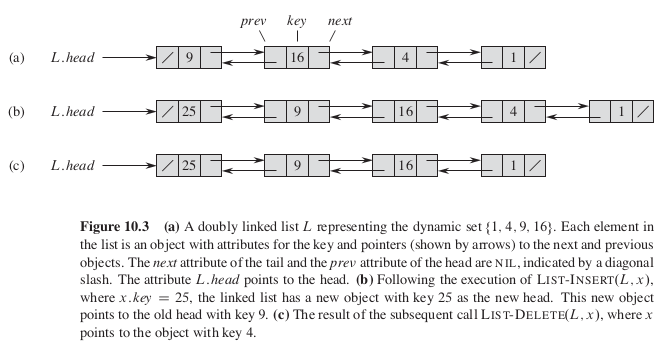
\includegraphics[width=.9\linewidth]{pics/c10_linked_list.png} \\

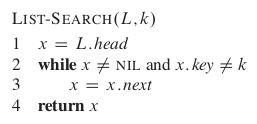
\includegraphics[width=.9\linewidth]{pics/c10_linked_list_search.png} \\

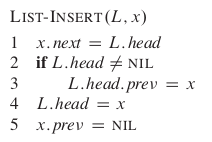
\includegraphics[width=.9\linewidth]{pics/c10_linked_list_insert.png} \\

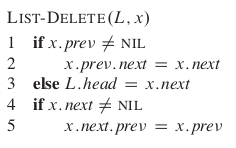
\includegraphics[width=.9\linewidth]{pics/c10_linked_list_delete.png} \\

The code for LIST-DELETE would be simpler if we could ignore the boundary conditions at the head and the tail of the list: \\

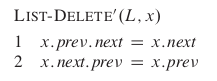
\includegraphics[width=.9\linewidth]{pics/c10_linked_list_delete2.png} \\

A sentinel is a dummy object that allows us to simplify boundary conditions. \\

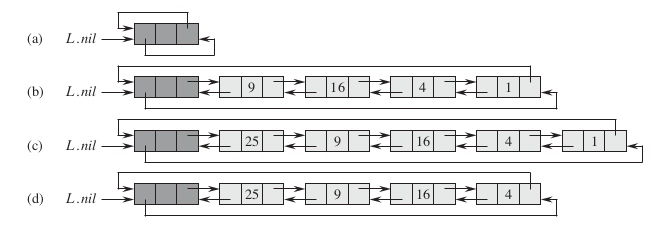
\includegraphics[width=.9\linewidth]{pics/c10_linked_list_2.png} \\

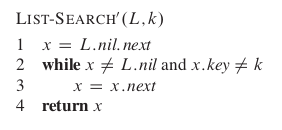
\includegraphics[width=.9\linewidth]{pics/c10_linked_list_search_2.png} \\

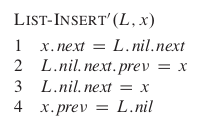
\includegraphics[width=.9\linewidth]{pics/c10_linked_list_insert_2.png} \\

Sentinels rarely reduce the asymptotic time bounds of data structure operations, but they can reduce constant factors. \\

selection probelm: \\
Input: A set of n (distinct) numbers and an interger i, with $1\le i\ge n$. \\
Output: The elements $x \in A$ that is larger than exactly i-1 other elements of A. \\


\begin{enumerate}
\item Minimum and maximum
\label{sec-4-1-2-1}
\begin{verbatim}
MINIMUM(A)
    min = A[1]
    for i = 2 to A.length
        if min > A[i]
            min = A[i]
    return min
\end{verbatim}


\begin{verbatim}
MIN_MAX(A)
    # init the min and max and start index
    if A.lenght is odd
        min = A[1]
        max = A[1]
        start = 2
    else
        if A[1] > A[2]
            min = A[2]
            max = A[1]
        else
            min = A[1]
            max = A[2]
        start = 3

    for i = start to A.length by 2
        if A[i] > A[i + 1]
            if A[i] > max
                max = A[i]
            if A[i + 1] < min
                min = A[i + 1]
        else
            if A[i + 1] > max
                max = A[i + 1]
            if A[i] < min
                min = A[i]
    
    return min, max
\end{verbatim}

\item Selection in expected linear time
\label{sec-4-1-2-2}
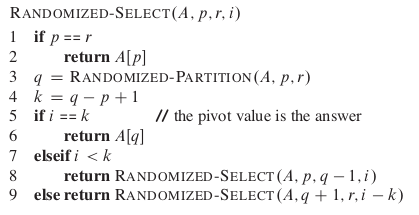
\includegraphics[width=.9\linewidth]{pics/c9_randomized_select.png} \\

\item Selection in worst-case linear time
\label{sec-4-1-2-3}
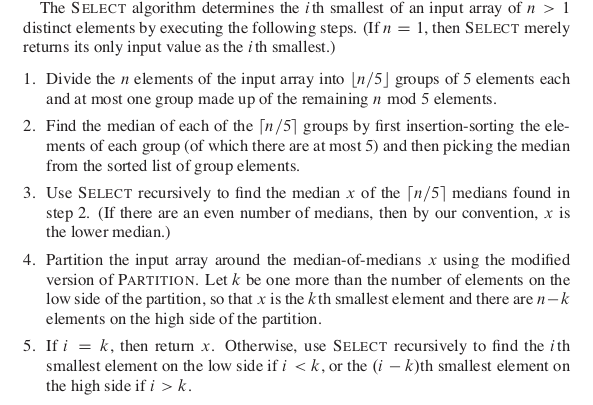
\includegraphics[width=.9\linewidth]{pics/c9_select.png} \\
\end{enumerate}



\subsubsection{Representing rooted trees}
\label{sec-4-1-3}

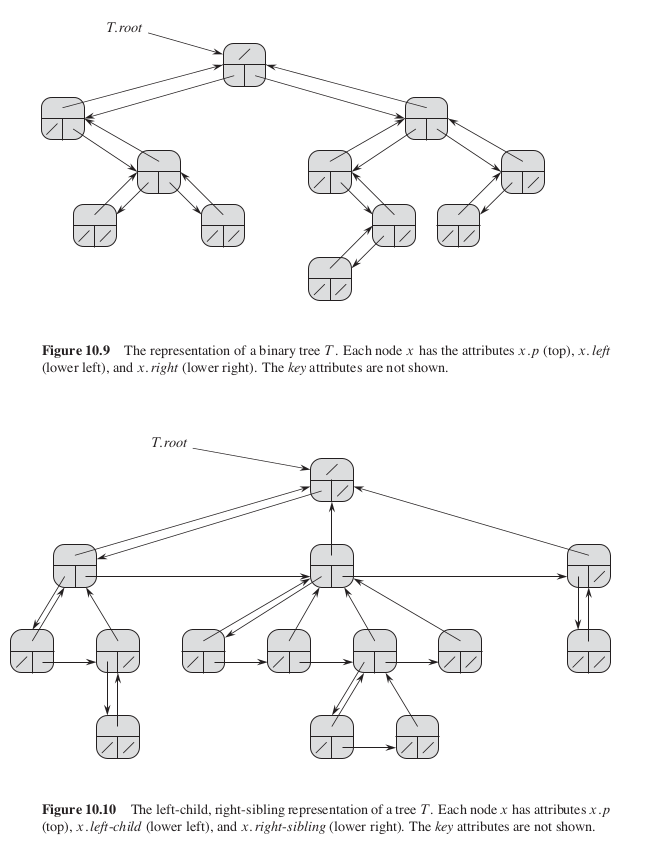
\includegraphics[width=.9\linewidth]{pics/c10_rooted_tree.png} \\

\subsection{Hash Tables}
\label{sec-4-2}
Many applications require a dynamic set that supports only the dictionary operations INSERT, SEARCH, and DELETE. \\

Directly addressing into an ordinary array makes effective use of our ability to examine an arbitrary position in an array in O(1) time. \\

When the number of keys actually stored is small relative to the total number of possible keys, hash tables become an effective alternative to directly addressing an array, since a hash table typically uses an array of size proportional to the number of keys actually stored. Instead of using the key as an array index directly, the array index is computed from the key. \\

\begin{verbatim}
Hashing is an extremely effective and practicaltechnique: 
the basic dictionary operations require only O(1) time on the average.
\end{verbatim}


\subsubsection{Direct-address tables}
\label{sec-4-2-1}
Direct addressing is a simple technique that works well when the universe U of keys is reasonably small. \\


To represent the dynamic set, we use an array, or direct-address table, denoted by T[0..m-1], in which each position, or slot, corresponds to a key in the universe U. \\

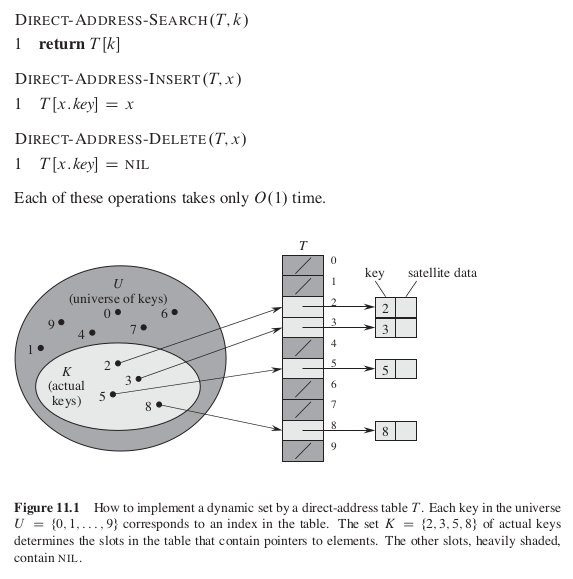
\includegraphics[width=.9\linewidth]{pics/c11_direct_address_table.png} \\

\subsubsection{Hash Tables}
\label{sec-4-2-2}
The downside of direct addressing is obvious: \\
\begin{enumerate}
\item if the universe U is large, storing a table T of size |U| may be impractical, or even impossible. \\
\item the set K of keys actually stored may be so small relative to U that most of the space allocated for T would be wasted. \\
\end{enumerate}


When the set K of keys stored in a dictionary is much smaller than the universe U of all possible keys, a hash table reduces the storage requirement to $\Theta(|K|)$ while maintains the benefit that searching for an element in the hash table still requires only O(1) time. \\


we use a hash function h to compute the slot from the key k. \\
\begin{equation}
h: U \rightarrow \{0,1,...,m-1\}
\end{equation}

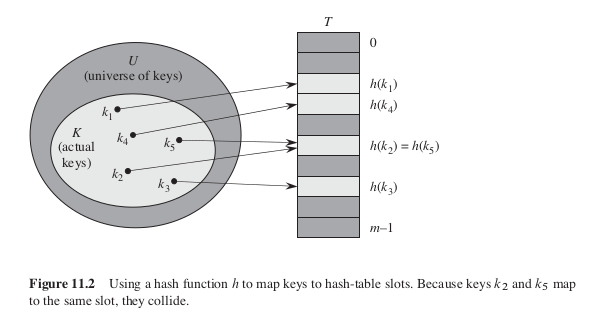
\includegraphics[width=.9\linewidth]{pics/c11_hash_table.png} \\

\begin{enumerate}
\item Collision resolution by chaining
\label{sec-4-2-2-1}
In chaining, we place all the elements that hash to the same slot into the same linked list. \\

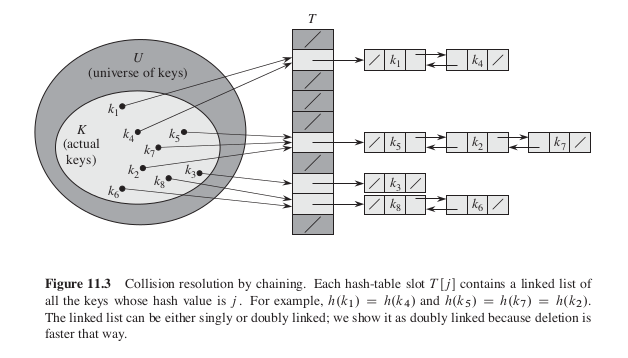
\includegraphics[width=.9\linewidth]{pics/c11_hash_table_chaining.png} \\

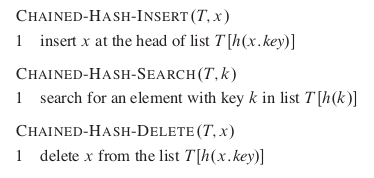
\includegraphics[width=.9\linewidth]{pics/c11_hash_table_chaining_psudo.png} \\


Given a hash table T with m slots that stores n elements, we define the load factor $\alpha$ for T as n/m, that is, the average number of elements stored in a chain. \\

simple uniform hashing: \\
Any given element is equally likely to hash into any of the m slots, independently of where any other element has hashed to. \\
\end{enumerate}

\subsubsection{Hash Functions}
\label{sec-4-2-3}
A good hash function satisfies (approximately) the assumption of simple uniform hashing: each key is equally likely to hash to any of the m slots, independently of where any other key has hashed to. \\

In practice, we can often employ heuristic techniques to create a hash function that performs well. \\

A good approach derives the hash value in a way that we expect to be independent of any patterns that might exist in the data. \\

Most hash functions assume that the universe of keys is the set $N={0,1,2,...}$ of natural numbers. Thus, if the keys are not natural numbers, we find a way to interpret them as natural numbers. \\

\begin{enumerate}
\item The division method
\label{sec-4-2-3-1}
h(k) = k mod m \\

\begin{verbatim}
m should not be a power of 2, since if m = 2^p , then h(k) is just the p lowest-order bits of k.
A prime not too close to an exact power of 2 is often a good choice for m.
\end{verbatim}
\item The multiplication method
\label{sec-4-2-3-2}
$h(k) = \lfloor m(kA\ \mathbb{mod}\ 1) \rfloor$ \\
$A \approx (\sqrt{5} - 1)/2$ \\
\end{enumerate}
\subsubsection{Open addressing}
\label{sec-4-2-4}

\subsection{Binary Search Trees}
\label{sec-4-3}

\subsubsection{What is a binary search tree?}
\label{sec-4-3-1}
A binary search tree is organized in a binary tree. \\

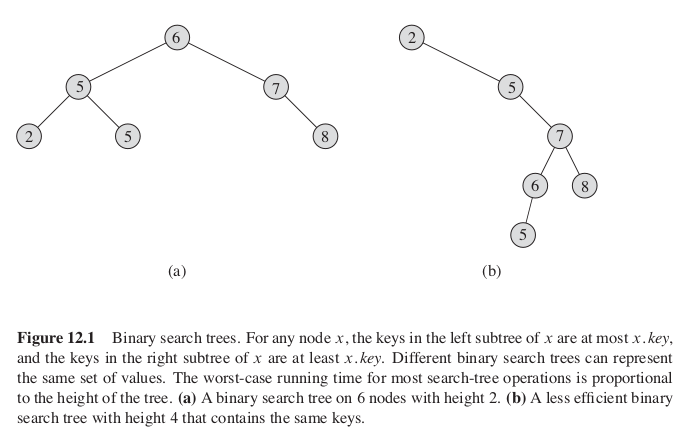
\includegraphics[width=.9\linewidth]{pics/c12_binary_search_tree.png} \\

binary-search-tree property: \\
Lets $x$ be the node in a binary search tree. If $y$ is a node in the left subtree of $x$, then $x.key \le x.key$. If $y$ is a node in the right subtree of $x$, then $y.key \ge x.key$. \\

The binary-search-tree property allows us to print out all the keys in a binary search tree in sorted order by a simple recursive algorithm, called an inorder tree walk. This algorithm is so named because it prints the key of the root of a subtree between printing the values in its left subtree and printing those in its right subtree. \\


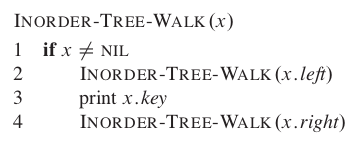
\includegraphics[width=.9\linewidth]{pics/c12_inorder_tree_walk.png} \\


If x is the root of an n-node subtree, then the call INODER-TREE-WALK(x) takes $\Theta(n)$ time. \\

\subsubsection{Querying a binary search time}
\label{sec-4-3-2}
SEARCH, MINIMUM, MAXIMUM, SUCCESSOR, PREDECESSOR run in O(h) time. (h is the height) \\

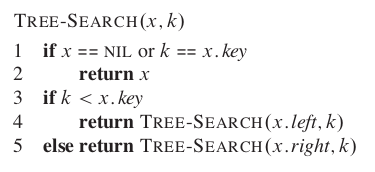
\includegraphics[width=.9\linewidth]{pics/c12_tree_search.png} \\

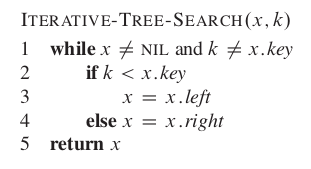
\includegraphics[width=.9\linewidth]{pics/c12_iterative_tree_search.png} \\

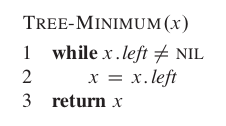
\includegraphics[width=.9\linewidth]{pics/c12_tree_minimum.png} \\

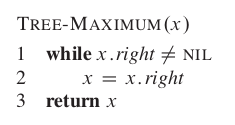
\includegraphics[width=.9\linewidth]{pics/c12_tree_maximum.png} \\

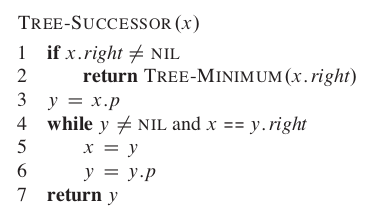
\includegraphics[width=.9\linewidth]{pics/c12_tree_successor.png} \\

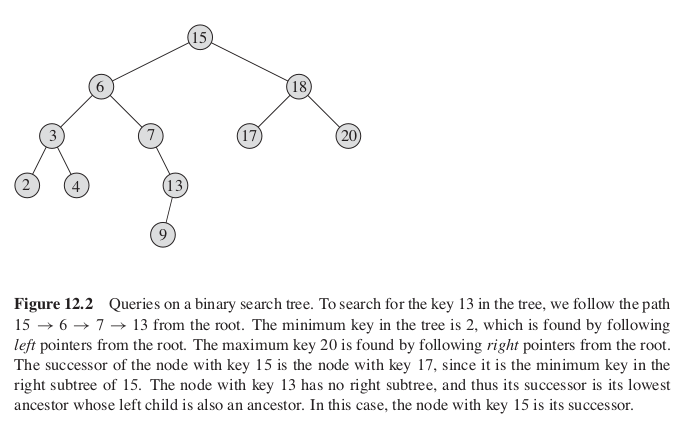
\includegraphics[width=.9\linewidth]{pics/c12_search_fig.png} \\

\begin{verbatim}
TREE-PREDECESSOR(x)
  if x.left != NIL
    return TREE-MINIMUM(x.left)
  y = x.p
  while y != NIL and x == y.left
    x = y
    y = y.p
  return y
\end{verbatim}

\begin{verbatim}
If a node in a binary search tree has two children, then its successor has no left child and its predecessor has no right child.
(Ohterwise it will be successor or predecessor)
\end{verbatim}

\subsubsection{Insertion and deletion}
\label{sec-4-3-3}
INSERTION and DELETION run in O(h) time. \\

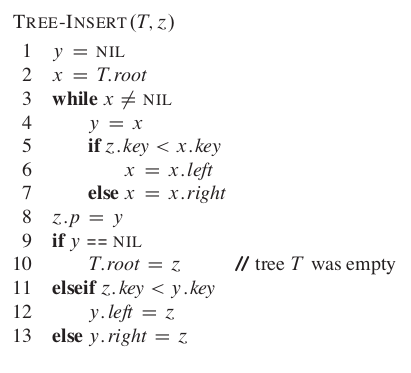
\includegraphics[width=.9\linewidth]{pics/c12_tree_insert.png} \\

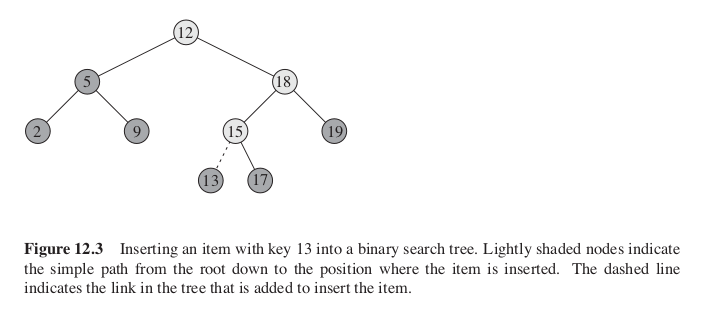
\includegraphics[width=.9\linewidth]{pics/c12_tree_insert_fig.png} \\


deletetion auxilary function: \\

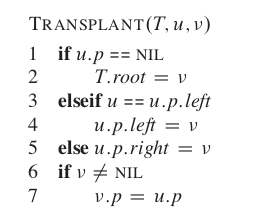
\includegraphics[width=.9\linewidth]{pics/c12_transplant.png} \\


\includegraphics[width=.9\linewidth]{pics/c12_tree_delete_fig.jpeg} \\

\includegraphics[width=.9\linewidth]{pics/c12_tree_delete.jpeg} \\


\subsection{Red-Black Trees}
\label{sec-4-4}
Red-black trees are one of many search-tree schemes that are "balanced" in order to guarantee that basic dynamic-set operations take $O(\lg n)$ time in the worst case. \\

\subsubsection{Properties of red-black trees}
\label{sec-4-4-1}

A red-black tree is a binary search tree with one extra bit of storage per node: its color, which can be either RED or BLACK . By constraining the node colors on any simple path from the root to a leaf, red-black trees ensure that no such path is more than twice as long as any other, so that the tree is approximately balanced. \\

\begin{verbatim}
Red-black properties:
1. Every node is either red or black.
2. The root is black.
3. Every leaf ( NIL ) is black.
4. If a node is red, then both its children are black.
5. For each node, all simple paths from the node to descendant leaves contain the same number of black nodes.
\end{verbatim}

\includegraphics[width=.9\linewidth]{pics/c13_red_black_tree_fig.png} \\


As a matter of convenience in dealing with boundary conditions in red-black tree code, we use a single sentinel to represent NIL. We use the sentinel so that we can treat a NIL child of a node x as an ordinary node whose parent is x. \\

\textbf{black-height} of the node: (denoted bh(x)) \\
the number of black nodes on any simple path from, but not including, a node x down to a leaf \\



Lemma: \\
A red-black tree with n internal nodes has height at most $2\lg(n+1)$. \\

\subsubsection{Rotations}
\label{sec-4-4-2}
ratation: a local operation in a search tree that preserves the binary-search-tree property. (run in O(1) time) \\

\includegraphics[width=.9\linewidth]{pics/c13_left_rotate.jpeg} \\


\subsubsection{Insertion}
\label{sec-4-4-3}

\includegraphics[width=.9\linewidth]{pics/c13_insert.png} \\

\includegraphics[width=.9\linewidth]{pics/c13_insert_fixup.png} \\

To understand how RB-INSERT-FIXUP works, we break the code into 3 major steps. \\
\begin{enumerate}
\item determine the violations of the red-black properties \\
\item examine the overall goal of the while loop \\
\item explore each of the three cases \\
\end{enumerate}

\includegraphics[width=.9\linewidth]{pics/c13_insert_fixup_fig.png} \\


\subsubsection{Deletion}
\label{sec-4-4-4}
\includegraphics[width=.9\linewidth]{pics/c13_rb_transplant.png} \\

\includegraphics[width=.9\linewidth]{pics/c13_rb_delete.png} \\

\begin{verbatim}
y: as the node either removed from the tree or moved within the tree;
x: moves into node y's original position;
node y's color might change, the variable y-original-color stores y's color before any changes occur;
\end{verbatim}

\includegraphics[width=.9\linewidth]{pics/c13_rb_delete_fixup.png} \\

\includegraphics[width=.9\linewidth]{pics/c13_rb_delete_fixup_fig.png} \\

\begin{verbatim}
If y is red, the red-black properties still hold when y is removed or moved

If node y was black, three problems may arise:
1. y had been the root and a red child of y because the new root (property 2 violated)
2. if both x and x.p are red (property 4 violated)
3. moving y within the tree causes any simple path that privously contained y to have one fewer black node (property 5 violated)
\end{verbatim}

We can correct the violation of property 5 by saying that node x, now occupying y’s original position, has an "extra" black. That is, if we add 1 to the count of black nodes on any simple path that contains x, then under this interpretation, property 5 holds. When we remove or move the black node y, we “push” its blackness onto node x. The problem is that now node x is neither red nor black, thereby violating property 1. \\


\subsection{Augmenting Data Structures}
\label{sec-4-5}

\subsubsection{Dynamic order statistics}
\label{sec-4-5-1}
An order-statistic tree T is simply a red-black tree with additional information stored in each node. \\

\includegraphics[width=.9\linewidth]{pics/c14_os_tree.png} \\
Besides the usual red-black tree attributes x.key, x.color, x.p, x.left, and x.right in a node x, we have another attribute, x.size. This attribute contains the number of (internal) nodes in the subtree rooted at x (including x itself), that is, the size of the subtree. \\

\begin{enumerate}
\item Retrieving an element with a given rank
\label{sec-4-5-1-1}
\includegraphics[width=.9\linewidth]{pics/c14_os_select.png} \\

\item Determing the rank of an element
\label{sec-4-5-1-2}
\includegraphics[width=.9\linewidth]{pics/c14_os_rank.png} \\

\item Maintaing subtree sizes
\label{sec-4-5-1-3}
\end{enumerate}

\subsubsection{How to augment a data structure}
\label{sec-4-5-2}
We can break the process of augmenting a data structure into four steps: \\
\begin{enumerate}
\item Choose an underlying data structure. \\
\item Determine additional information to maintain in the underlying data structure. \\
\item Verify that we can maintain the additional information for the basic modifying operations on the underlying data structure. \\
\item Develop new operations. \\
\end{enumerate}

\begin{verbatim}
As with any prescriptive design method, you should not blindly follow the steps
in the order given. Most design work contains an element of trial and error, and
progress on all steps usually proceeds in parallel. There is no point, for example, in
determining additional information and developing new operations (steps 2 and 4)
if we will not be able to maintain the additional information efficiently. Neverthe-
less, this four-step method provides a good focus for your efforts in augmenting
a data structure, and it is also a good way to organize the documentation of an
augmented data structure.
\end{verbatim}


Theroem (augmenting a red-black tree) \\
\begin{verbatim}
Let f be an attribute that augments a red-black tree T of n nodes, and suppose that
the value of f for each node x depends on only the information in nodes x, x.left,
and x.right, possibly including x.left.f and x.right.f. Then, we can maintain the
values of f in all nodes of T during insertion and deletion without asymptotically
affecting the O(lgn) performance of these operations.
\end{verbatim}

\subsubsection{Interval trees}
\label{sec-4-5-3}
A closed interval is an ordered pair of real numbers $[t_1, t_2]$ with $t_1 \le t_2$ . The interval $[t_1, t_2]$ represents the set $\{t \in \mathbb{R}: t_1 \le t \le t_2\}$. \\

Any two intervals $i$ and $i'$ satisfy the interval trichotomy; that is, exactly one of the following three properties holds: \\
\begin{enumerate}
\item $i$ and $i'$ overlap \\
\item $i$ is to the left of $i'$ \\
\item $i$ is to the right of $i'$ \\
\end{enumerate}

An interval tree is a red-black tree that maintains a dynamic set of elements, with each element x containing an interval x.int. \\

Interval trees support the following operations: \\
\includegraphics[width=.9\linewidth]{pics/c14_interval_tree_op.png} \\

\includegraphics[width=.9\linewidth]{pics/c14_interval_tree_fig.png} \\

\includegraphics[width=.9\linewidth]{pics/c14_interval_search.png} \\
\section{Advanced Design and Analysis Techniques}
\label{sec-5}
Dynamic programming typically applies to optimization problems in which we make a set of choices in order to arrive at an optimal solution. As we make each choice, subproblems of the same form often arise. Dynamic programming is effective when a given subproblem may arise from more than one partial set of choices; the key technique is to store the solution to each such subproblem in case it should reappear. \\

Greedy algorithms typically apply to optimization problems in which we make a set of choices in order to arrive at an optimal solution. The idea of a greedy algorithm is to make each choice in a locally optimal manner. \\

We use amortized analysis to analyze certain algorithms that perform a sequence of similar operations. Instead of bounding the cost of the sequence of operations by bounding the actual cost of each operation separately, an amortized analysis provides a bound on the actual cost of the entire sequence. One advantage of this approach is that although some operations might be expensive, many others might be cheap. \\
\subsection{Dynamic Programming}
\label{sec-5-1}
Dynamic programming solves problems by combining the solutions to subproblems. ("programming" in this context refers to a tabular method, not to writing computer code.) \\
Dynamic programming applies when the subproblems overlap. \\
A dynamic programming algorithm solve each subproblem just once and then save its answer in a table, thereby avoiding the work of recomputing the answer every time is solves each subproblem. \\

We typically apply dynamic programming to optimization problems. \\

When developing a dynamic programming algorithm, we follow a sequence of four steps: \\
\begin{enumerate}
\item characterize the structure of an optimal solution \\
\item recursivly define the value of an optimal solution \\
\item compute the value of an optimal solution, typically in a bottom-up fashion \\
\item construct an optimal solution from computed information \\
\end{enumerate}
\subsubsection{Rod cutting}
\label{sec-5-1-1}
The rod-cutting problem: \\
Given a rod of length n inches and a table of price $p_i$ for $i=1,2,...,n$, determine the maximum revenue $r_n$ obtainable by cutting up the rod and selling the pieces. \\

We can cut up a rod of length $n$ in $2^{n-1}$ different ways. \\

\includegraphics[width=.9\linewidth]{pics/c15_rod_cutting1.png} \\

\includegraphics[width=.9\linewidth]{pics/c15_rod_cutting2.png} \\

If an optimal solution cuts the rod into k pieces, for some $1\le k \le n$, then an optimal decomposition \\
$n = i_1 + i_2 + ... + i_k$ \\
of the rod into pieces of lengths $i_1,i_2,...,i_k$ provides maximum corresponding revenue \\
$r_n = p_{i_1} + p_{i_2} + ... + p_{i_k}$. \\

Frame the values $r_n$ for $n\ge 1$ in terms of optimal revenues from shorter rods: \\
\begin{equation}
r_n = \max(p_n, r_1+r_{n-1}, r_2+r_{n-2},...,r_{n-1}+r_1)
\end{equation}


To solve the original problem of size $n$, we solve smaller problems of the same type, but of smaller sizes. The overall optimal solution incorporates optimal solution to the two related subproblems, maximizing revenue from each of those two pieces. \\

We say that the rod-cutting problem exhibits \textbf{optimal substructure}: optimal solutions to a problem incorporate optimal solutions to related subproblems, which we may solve independently. \\


In a related, but slightly simpler, way to arrange a recursive structure for the rod-cutting problem, we view a decomposition as consisting of a first piece of length $i$ cut off the left-hand end, and then a right-hand remainder of length $n-i$. Only the remainder, and not the first piece, may be further divided. We thus obtain the following simpler version: \\
\begin{equation}
r_n = \max_{1\le i \le n}(p_i + r_{n-i}).
\end{equation}

In this formulation, an optimal solution embodies the solution to only one related subproblem—the remainder—rather than two. \\
\begin{enumerate}
\item Recursive top-down implementation
\label{sec-5-1-1-1}

\includegraphics[width=.9\linewidth]{pics/c15_cut_rod.png} \\


\begin{verbatim}
Why is CUT-ROD so inefficient? 
The problem is that CUT-ROD calls itself recursively over and over 
again with the same parameter values; it solves the same subproblems 
repeatedly.
\end{verbatim}
\item Using dynamic programming for optimal rod cutting
\label{sec-5-1-1-2}
The dynamic-programming method works as follows. Having observed that a naive recursive solution is inefficient because it solves the same subproblems repeatedly, we arrange for each subproblem to be solved only once, saving its solution. Dynamic programming thus uses additional memory to save computation time; it serves an example of a time-memory trade-off. The savings may be dramatic: an exponential-time solution may be transformed into a polynomial-time solution. A dynamic-programming approach runs in polynomial time when the number of distinct subproblems involved is polynomial in the input size and we can solve each such subproblem in polynomial time. \\
\end{enumerate}
% Emacs 25.2.1 (Org mode 8.2.10)
\end{document}
